% !TeX root = 190227.tex
\section{Использование библиотек}
\begin{frame}[t]{Разделение на модули}
	\begin{itemize}
	\item
		В большой программе "--- много кода
	\item
		Например, в игре:
		\begin{itemize}
		\item Отрисовка графики
		\item Звук
		\item Управление персонажем
		\item Отслеживание прогресса на уровне и жизней
		\item ИИ для мобов
		\item Многопользовательский режим
		\end{itemize}
	\item
		Всё писать в одном файле неудобно
	\item
		В нескольких случайных файлах тоже неудобно
	\item
		Делят на модули "--- логические куски.
	\end{itemize}
\end{frame}

\begin{frame}[t]{Зацепление и связность}
	\begin{center}
		\includegraphics[height=0.8\textheight,keepaspectratio]{CouplingVsCohesion.pdf}
	\end{center}
\end{frame}

\begin{frame}[t]{Библиотеки}
	\begin{itemize}
	\item
		Библиотека "--- набор готовых функций, классов и прочего,
		в Python обычно пакуется в несколько пакетов/модулей
	\item
		Принимает за вас какие-то решения и предлагает
		свой взгляд на мир (<<как работать с массивами>>)
	\item
		Если взгляд совпал "--- использовать удобно
	\item
		У больших/популярных библиотек обязательно читать
		документацию и вводное руководство, чтобы проникнуться
		взглядом на мир
	\item
		Язык полезен не сам по себе, а доступными библиотеками
		на любой случай жизни\footnote{\href{https://github.com/vinta/awesome-python}{github.com/vinta/awesome-python}, есть и для других языков}
	\item
		Библиотека может строиться на других библиотеках (\textit{зависимости})
	\end{itemize}
\end{frame}

\begin{frame}[t]{Дистрибьюция библиотек}
	\begin{itemize}
		\item Раньше: идём на сайт, качаем, устанавливаем
		\item Теперь модно: свой пакетный менеджер и центральный репозиторий
		\item Для Python: PyPI\footnote{Например, \href{https://pypi.org/project/pytest/}{pypi.org/project/pytest/}}, для Java "--- Maven Central, для NodeJS "--- NPM
		\item Обычно ничего скачивать руками или компилировать не надо, всё само
		\item Премодерации нет, \href{могут быть вирусы}{https://www.opennet.ru/opennews/art.shtml?num=49490}
		\item Компании могут сделать свои репозитории (для внутренних библиотек)
		\item Интересно (не) сочетается с системным пакетным менеджером (apt-get)
	\end{itemize}
\end{frame}

\begin{frame}[t,fragile]{Куда устанавливать библиотеки}
	Глобальная (системная) установка:
	\begin{itemize}
		\item Можно использовать везде \textit{на конкретной машине}
		\item Используется ровно одна версия библиотеки $\Rightarrow$ сложности с зависимостями
		\item Если есть системный пакетный менеджер, то ему плохо
		\item Сложно отследить, что написанному коду реально надо ставить
	\end{itemize}
	Ещё иногда можно ставить <<для конкретного пользователя>>.
	
	В Python есть virtualenv:
	\begin{itemize}
		\item Создаётся отдельное <<окружение>> в папке со своей копией питона и
			независимым набором библиотек
		\item
			Для активизации набираем \verb`source some_env/Scripts/activate`
			или выбираем SDK
		\item В это окружение можно ставить что угодно независимо от глобального
		\item Изолирует код, легко отследить зависимости и версии
	\end{itemize}
\end{frame}

\begin{frame}[t,fragile]{На практике}
	Пока пишете <<на коленке>> "--- можно ставить глобально.
	
	Rules of thumb:
	\begin{itemize}
	\item
		Никогда не запускайте \verb`setup.py` или \verb`easy_install`
	\item Windows: используйте Anaconda и \verb`conda install` или \verb`pip install` (от имени Администратора)
	\item Linux (Ubuntu): системный пакетный менеджер и пакеты вроде \verb`python3-pytest` либо virtualenv
		\begin{itemize}
		\item Никогда не делать \verb`sudo pip install`!
		\end{itemize}
	\item macOS: для конкретного пользователя: \verb`brew install python` и `pip install`
	\item Не используйте virtualenv
	\item Не надейтесь, что удастся поставить не последнюю версию библиотеки
	\item На надейтесь на непопулярные библиотеки
	\end{itemize}
\end{frame}

\begin{frame}[t]{Как выбрать библиотеку}
	\begin{enumerate}
	\item Проверить Awesome Python и погуглить
	\item Недавние и регулярные релизы, тысячи звёзд на GitHub, приличный README и документация на readthedocs.org (для Python)
	\item Читаем getting started/tutorial/handbook и смотрим на примеры: нравится ли синтаксис
	\item Изучить ещё несколько библиотек
	\item Ставим библиотеку
	\item Проходим getting started/tutorial/handbook и руками набираем все примеры, чтобы проникнуться идеологией и предметной областью
	\item Когда надо решить конкретную задачу "--- гугл, StackOverflow, документация\label{sodriven}
	\end{enumerate}
	
	Не стоит начинать с пункта \ref{sodriven}, будет StackOverflow-Driven Development, код будет не поменять.
\end{frame}

\begin{frame}[t]{Практика: поиск библиотеки для картинок}
	Задача: есть картинка JPG, надо на ней нарисовать текст.
	
	Какие есть библиотеки?
\end{frame}

\begin{frame}[t]{Библиотеки для работы с картинками}
	OpenCV:
	\begin{itemize}
	\item Библиотека компьютерного зрения, но рисовать умеет
	\item Написана на плюсах, есть binding к Python и ещё куче языков
	\item Если ставить руками "--- надо компилировать плюсы так,
		чтобы было совместимо с конкретно вашим питоном (боль)
	\item Если ставить через пакетный менеджер "--- будет удобно
		(особенно под Linux)
	\item Документация и примеры в основном на плюсах, но Python пытается подражать
	\end{itemize}
	
	Pillow:
	\begin{itemize}
	\item Развитие PIL (Python Imaging Library) для Python 3
	\item Алгоритмов компьютерного зрения нет, есть картинки
	\item Например, умеет выбирать шрифт для надписи
	\end{itemize}
\end{frame}

\begin{frame}{Особенности отрисовки текста}
	\begin{center}
		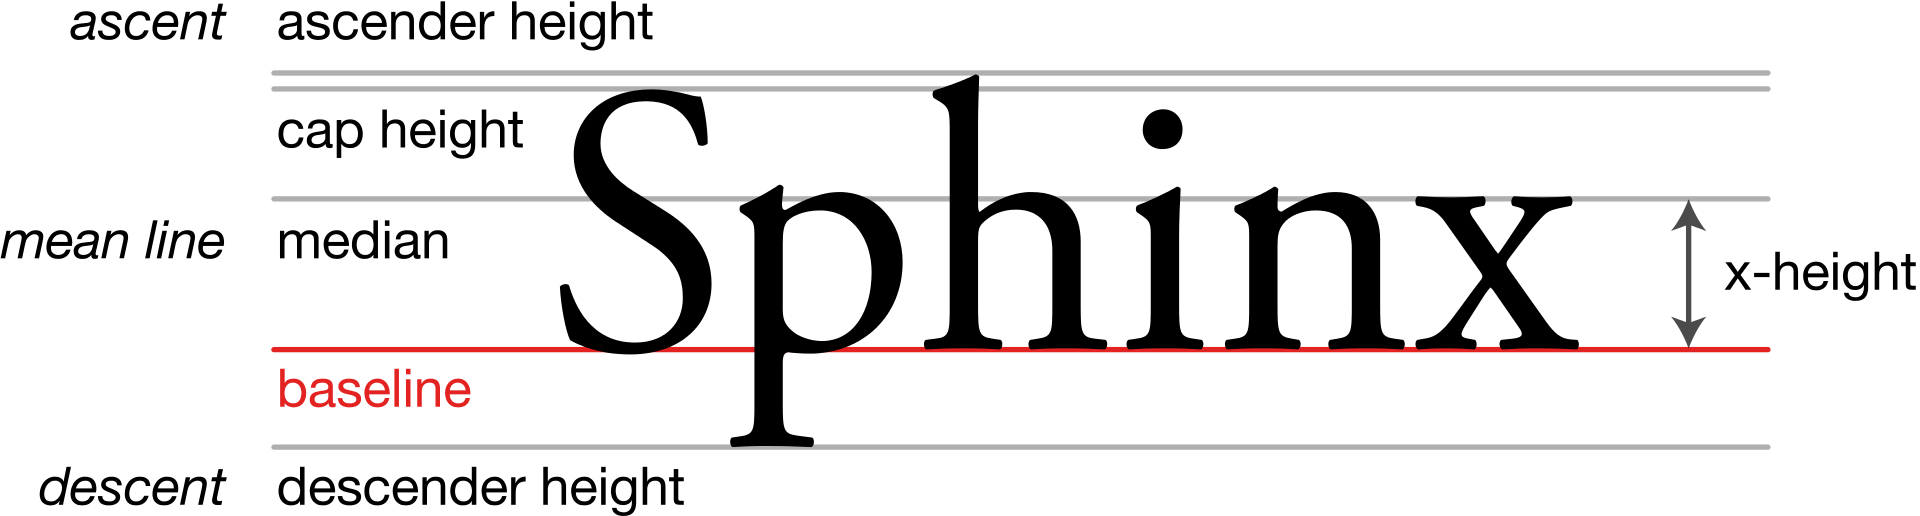
\includegraphics[width=\linewidth,keepaspectratio]{typography.png}
	\end{center}
	
	Чтобы текст выглядел <<ровно>>, надо отрисовывать с одинаковой
	$y$-координатой у baseline, а не левого нижнего угла.
\end{frame}

\begin{frame}[t]{Научные библиотеки}
	\begin{itemize}
	\item SymPy "--- символьные вычисления (возьмите интеграл от $x^3$)
	\item NumPy "--- быстрая работа с данными (написана на плюсах)
	\item Pandas "--- удобный NumPy
	\item seaborn, matplotlib "--- визуализация данных
	\item scikit-learn "--- машинное обучение
	\end{itemize}
\end{frame}
